\documentclass[12pt]{article}

\usepackage{amssymb,amsmath}
\usepackage{geometry}
\usepackage{fancyhdr}
\usepackage{lastpage}
\usepackage{graphicx}
\usepackage{epstopdf}
\usepackage{epsfig}
\usepackage{slashed}
\usepackage{amsbsy}
\usepackage{color}
\usepackage{enumerate}
\usepackage[colorlinks = true, linkcolor = blue, urlcolor=blue,citecolor = blue]{hyperref}

%%\geometry{left=1in,right=1in,top=1in,bottom=1in}
%%\pagestyle{fancy}
%%\fancyhf{}
\fancyfoot[C]{-~\thepage ~-}

\numberwithin{equation}{section}

\begin{document}
\title{User's and Programmer's Guide for the Hall C One-Event Display (EVe)}
\author{Benjamin Davis-Purcell\\
McMaster University,\\
University of Regina\\
\texttt{davispbr@mcmaster.ca}}
\date{\today}
\maketitle
\begin{abstract}
EVe is a one-event display originally written by Miha Mihovilovic in 2008 for the Hall A BigBite Spectrometer. It has been modified to run for Hall C data and geometries, currently set up with the HMS geometry. EVe is a work in progress for Hall C as there are multiple issues that need to be fixed, but the underlying code is in place for the basics to run smoothly once a few corrections are completed. The current code can be cloned from github at \url{https://github.com/JeffersonLab/EVe\_HallC}. An tarball of the original BigBite code and its manual can be found at \url{https://github.com/JeffersonLab/EVe\_HallC/tree/master/Docs/EVe-BigBite}.

This document serves as an initial guide, describing how the Event Display works and outlining what each class and function does. It also points out the key things that need to be fixed to allow the display to become fully operational, and outlines further steps for improvement, suggesting ways to make such improvements. Some classes from the original version have not yet been altered or activated at all, aside from translating comments and variable names from Slovenian to English. Comments were kept as clear as possible, though there may be a couple translation errors.
\end{abstract}

\pagebreak
\tableofcontents
\pagebreak

\section{Introduction}
The goal of the event display is to show various views of the detector, displaying hits and tracks through each medium. Currently, the event display has three views: planar, 3D, and projection. Each view still needs work to become fully operational. Once completed, the display has the ability to calculate and show full and partial tracks through the detector, along with roads-style tracking. Targets or other geometries can be drawn to be included in the tracking.

\section{Installation and Usage}
As was previously stated, the new version of EVe can be downloaded from github at \url{https://github.com/JeffersonLab/EVe\_HallC}. On this page, on the right-hand side where \textit{\textbf{HTTPS} clone URL} can be seen, copy the link underneath into the terminal. The command should look like this:
\\
\texttt{>> git clone https://github.com/JeffersonLab/EVe\_HallC.git }
\\
This will place the code in your current directory. Next, type \texttt{make} to compile the code. This creates a shared library \textit{libEVe.so} that is regenerated each compile. 
\\
\\
EVe must be run in the ROOT environment, either normal ROOT or the JLab/HallC analyzer. The version of ROOT should not matter, although the Hall C analyzer is currently based on ROOT 5.34/02, September 21, 2012, with CINT/ROOT C/C++ Interpreter version 5.18.00, July 2, 2010. It does not require any JLab-specific geometries at this point, although this could be added in later if one chooses. In order to run, EVe does require that \textit{TGClient.h} is included (\texttt{\#include <TGClient.h>}), and that the geometry file \textit{libGeom.so} gets loaded into root before usage. Once EVe has been \textit{made}, the self-generating EVe library \textit{libEVe.so} must also be loaded. The commands are as follows:
\\
\texttt{gSystem->Load("libGeom");} \\
\texttt{gSystem->Load("libEVe.so");}
\\
EVe can be run using a root macro, or opened directly from the root command line. The simplest way to open EVe is using the macro simEVe\_new.C, contained in the directory. This macro is used to analyze the \textit{hodtest.root} file that can be obtained from the Hall C 12GeV software Wiki, found \url{https://hallcweb.jlab.org/wiki/index.php/Analyzer/Running}. (The page will most likely need to be followed from \url{https://hallcweb.jlab.org/wiki/index.php/ROOT_Analyzer} though, which explains how to download the Hall C analyzer using git). Once the \textit{hodtest.root} file is located in the same directory as that which you have downloaded EVe into, you will be able to run \texttt{root} or \texttt{hcana}, followed by \texttt{.x simEVe\char`_new.C} in the root environment. This will start up EVe, analyzing the data in the hodtest root tree. The Event Display can easily be modified to read any incoming root file, though the branch addresses must match (or be modified within the code) in order to run correctly.
\\
If you are using EVe and updating code, thereby improving/changing the functionality of the display, please update this Manual as well; the \textit{.tex} file can be found in the EVe folder downloaded from github.

\section{Views}
There are currently 3 available views in the Event Display: Planar, 3D, and Projection, selectable via buttons on the display menu. They are briefly discussed in the following sections.

\subsection{Planar}
The planar view is used to show all detectors in 2D, looking directly at the detectors as an incoming particle would see them. Currently, the view shows all scintillator planes (hodoscopes) for the HMS (s1x, s1y, s2x, s2y) as well as the two HMS wire chambers. 
\\
\\
The PMTs on the scintillator planes light up when hit; a red hit means that only one PMT on that specific scintillator paddle was hit within the event time window, while green means that the 2 PMTs on either side of the scintillator paddle were hit for the same event (meaning a good hit). The layout and orientation still needs to be fixed for these planes; currently both \textit{y} planes are incorrect, as the paddles should be vertical and placed nicely in the canvas. Two different placement methods are shown to display the canvas tweaking. Possible corrections will be explained in a later section.
\\
\\
Wires in the wire chamber light up when hit, with each colour corresponding to a different wire plane. Tracks can be drawn through good hits in the wire chambers continuing through good hits in the hodoscopes. Currently, the tracking circles are set to the position (0,0) for each geometry piece to test out canvas locations, pinpointing one of the errors. The correct tracking ROOT tree branches are already loaded into the code, with the arrays currently being commented out.  
\\
\\
An image of the current planar view is shown in Figure \ref{fig:planar}.
\begin{figure}[h!]
	\caption{Sample of the EVe planar view. Scintillation planes and wire chambers can be seen with event hits. Tracking is turned on and set to the (0,0) position for each detector, showing the rotation error that must be corrected.} \label{fig:planar}
	\centering
	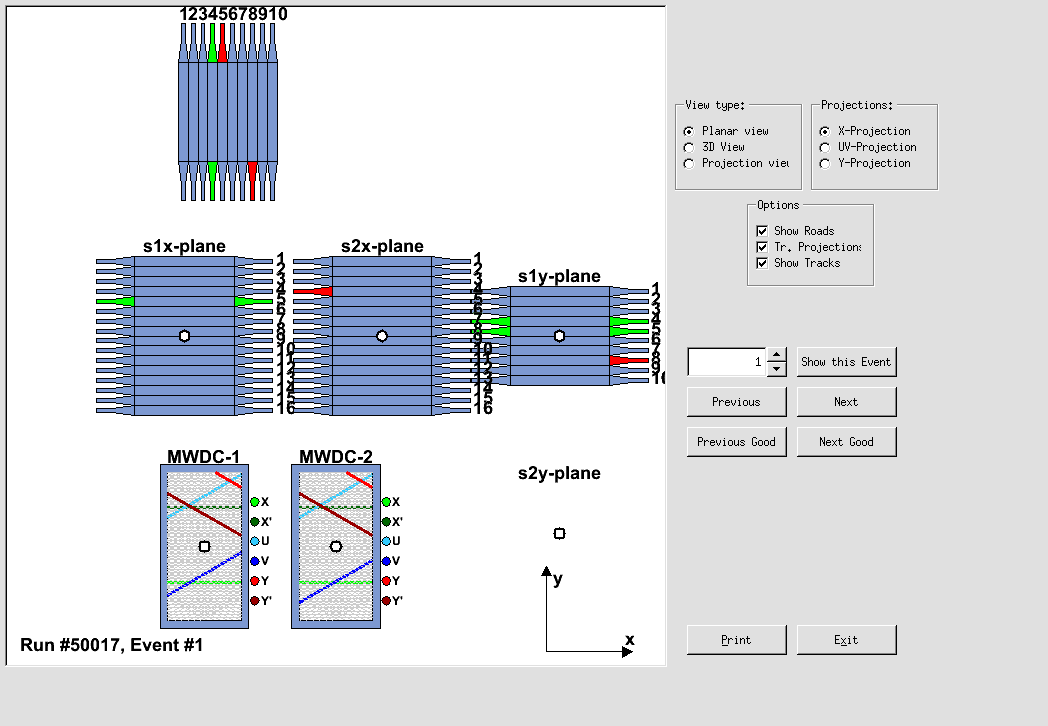
\includegraphics[width=0.9\textwidth]{PlanarView.png} 
\end{figure}  

\subsection{3D}
The 3D view is used to show all detectors in 3D, rotatable space. This is currently the view that is in its most raw form, as there are still large issues that need to be worked out. In the end, tracks can be drawn through all detectors, even originating from a target or beam which both can be drawn if one chooses to do so. This was done in the original BigBite version of the Event Display. Currently, tracking and hits need to be turned on for this view, but first the rotated s1y and s2y scintillator planes must have their PMTs drawn correctly and placed in the proper location. More details will follow in later sections.
\\
\\
An image of the current 3D view is shown in Figure \ref{fig:3D}.
\begin{figure}[h!]
	\caption{Sample of the EVe 3D view, which is fully ($4\pi$) rotatable. Wire chambers and hodoscopes can be seen.} \label{fig:3D}
	\centering
	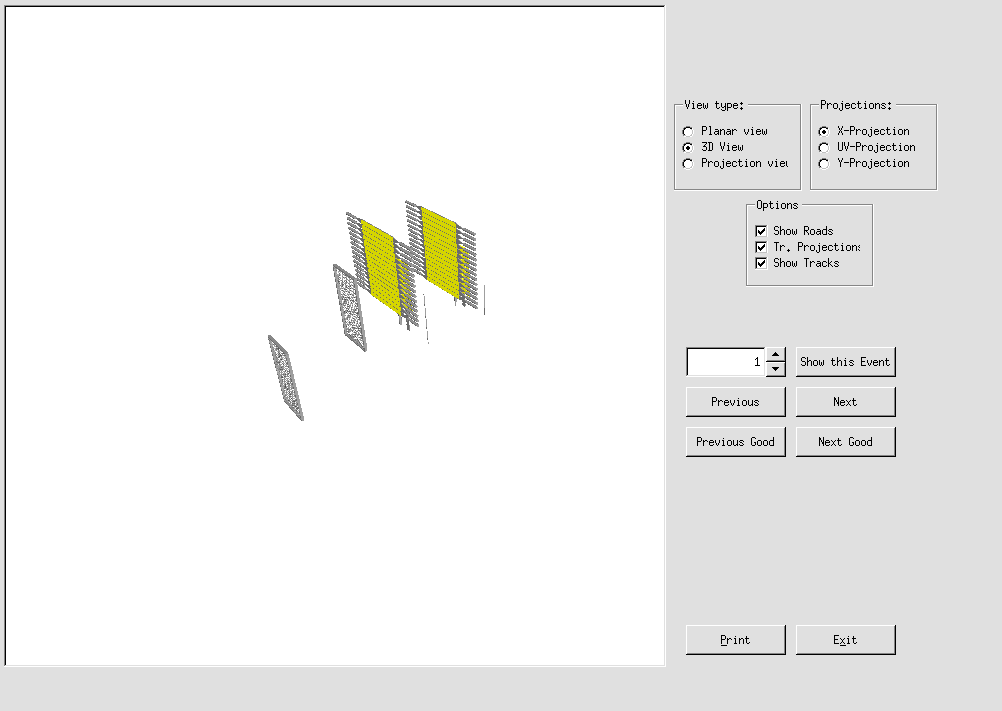
\includegraphics[width=0.9\textwidth]{3DView.png} 
\end{figure}  

\subsection{Projection} 
The projection view displays a bird's eye view of the wire chambers and tracks particles through the wire chambers, taking the time travelled into account along with wire number. The view shows both wire chambers, isolating a specific set of planes (i.e. X and X', U and V, Y and Y'). Here a red track means a hit on a front plane in a given wire chamber and a green track is the back plane. The length of the track line is given by the timing; a good track should be the same length in each corresponding chamber where a hit is found, as the drift time should be the same for a particle passing through both wire chambers. There is also an improved tracking feature available that is not yet implemented.
\\
\\
An image of the current projection view is shown in Figure \ref{fig:proj}.
\begin{figure}[h!]
	\caption{Sample of the EVe projection view.} \label{fig:proj}
	\centering
	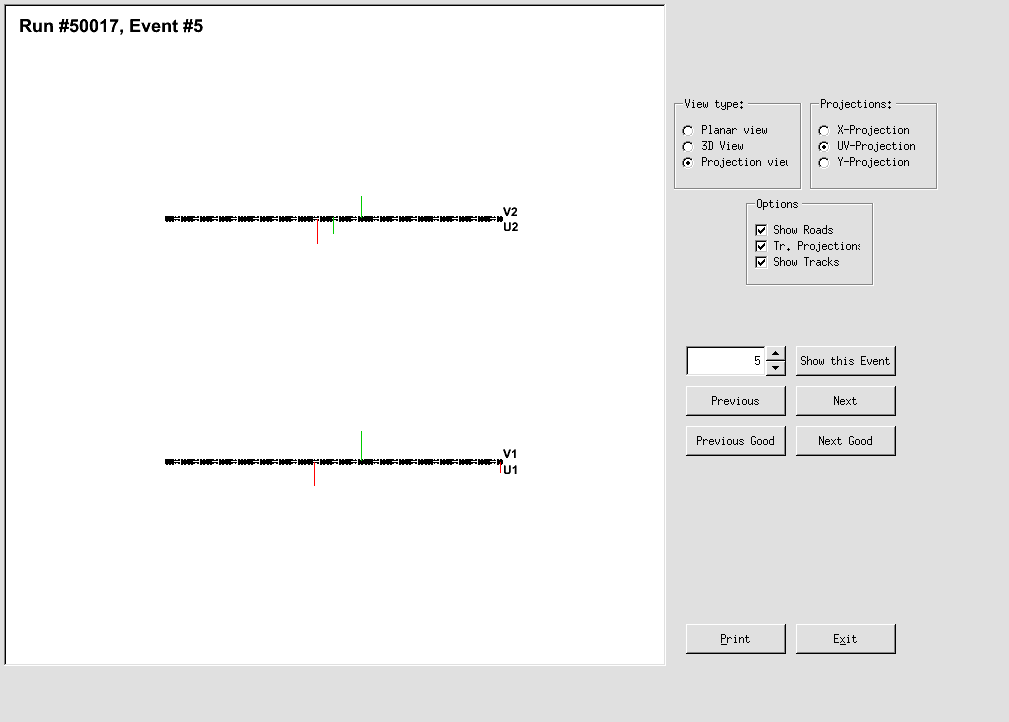
\includegraphics[width=0.9\textwidth]{ProjView.png} 
\end{figure} 

\section{Classes, Functions, and Special Files}
EVe is made up of many classes, which are brought together by the EVe.cxx class which creates the Event Display. Each class, aside from a few special cases, contains main code files (\textit{.cxx}) and header files (\textit{.h}). When compiled, object (\textit{.o}) and dependency (\textit{.d}) files are created.
\\
\\
This section will go through each class in varying detail, depending on how much the class was updated. In some cases, specific functions contained in a class will also be described. Only the \textit{.cxx} files will be specifically referred to (aside from the special cases). The classes will be appear in alphabetic order for neatness, with the special cases being left until the end (including the overarching EVe.cxx class).

\subsection{CStransform}
This class creates transformations that are used throughout the event display. These transformations convert SI units, i.e., metres, centimetres, etc., into canvas units, as in fractional location on the canvas. For example, in the x dimension, 0 would be the left edge of the canvas and 1 would be the right edge. Each time this class is called, it is initialized by creating a conversion ratio, 1/canvas\_length, as the key conversion factor which is used in each class function. The functions of this class simply perform the conversion in x, y, or length. This class is overloaded with 2 constructors; the second will only be initialized if 4 arguments are given. This was done as a test to try to correct the planar ScintPlane (the scintillation plane class) rotation, although it does not work as planned yet. 
\\
\\
This class is still not well-understood, as the planes did not rotate as hoped. This needs to be looked into more, especially with how it is used in the ScintPlane class. The CStransform for the ScintPlane class is created in EVe.cxx, of which one is currently called \texttt{s1y\_cst}.

\subsection{Detector3D}
The Detector3D class handles the entirety of the 3D view. All of the classes that combine to make up the 3D view, including MWDChamber3D and ScintPlane3D are instantiated within this class. This class is then neatly called in EVe.cxx, creating the 3D view.
\\
\\
There are some issues that must be resolved for this class involving the 3D scintillator planes. The y planes have vertical paddles; currently the PMTs for these paddles are not being drawn correctly. This is a problem in rotation and translation in the building of the paddles that is carried from this class to ScintPlane3D to ScintillatorPaddle3D and must be resolved. When this is fixed, tracking will be able to be correctly turned on. Hit detection still needs to be written using the exact same methods as are currently employed for 2D hits in the EVe.cxx, ScintPlane, and ScintillatorPaddle classes.

\subsection{FullTrajectory3D}
This class is used to draw complete tracks in 3D view. It can take into account any targets/magnets and/or other geometry objects that are included in the 3D geometry but do not contain hits, and use these objects to carry the tracking through from the target to the final detector.
\\
This class has not yet been tested in the new version of EVe and has not yet been set up to work properly. The code is unchanged from the original version.

\subsection{GetVariables}
The GetVariables class was written so that variables (ex. geometry variables) could be dynamically called from a text file to be used anywhere in EVe. When this class is instantiated, it takes in a text file. This is the file that contains all geometry information. Currently, the test file used is \textit{HMS.txt}. GetVariables then contains two functions that parse through the text file, searching for a specific string, for example, \textit{``Number of paddle PMTs = 2"}. All strings must end with a \textit{`= some\_number'} for the code to work. The functions take in this specific string and output a number to be used in the code. The GetVariables class does not necessarily need to be used, but was written as a means of cleaning up the code and allowing multiple variables to be input from multiple sources, instead of one geometry file.

\subsubsection{Function: GetDouble}
This function takes in a \textit{string} and outputs a \textit{double} variable. This is to be used whenever a non-integer is needed.

\subsubsection{Function: GetInt}
This function takes in a \textit{string} and outputs an \textit{integer} variable. In order for an integer variable to be input, this is the class that must be called. 

\subsection{MWDChamber}
This class is used to create planar wire chambers. When instantiated (inside EVe.cxx), it takes in a wire chamber name, wire number, width, height, canvas position, and type. A wire chamber is drawn with wires being created in each plane (eg. X, U, Y for wire chamber 1). Every 1 wire that is drawn on the canvas corresponds to 5 wires in the real detector, otherwise the display would be too messy (rounding occurs at the end, of course).
\\
\\
This class is one of a few that can be optimized by creating a sub-class which creates the method to draw a wire plane, which would then be called for each wire plane instead of copying and pasting code multiple times for each plane. 
\\
\\
This class contains functions for a wire hit for each different plane. A hit turns the wire that was hit a certain colour and bolds the line. A legend is also drawn and colour-matched for clarity. Tracking in this class is done by drawing circles over overlapping wires that could contain possible good tracks. The tracking still needs to be adjusted so that the canvas understands the real position being refereed to by the data in SI units. This probably relates to the issue that needs to be worked out with CStransform.

\subsection{MultiRoads}
This class creates multi roads for the projection view. It is completely unaltered from the original code and has not been activated yet in the new version, therefore it still needs to be tested with the right data.

\subsection{Road}
This class creates roads for the projection view. Like MultiRoads, it has not been altered, nor has it been activated or tested.

\subsection{ScintPlane}
This class creates a scintillation plane in the planar view. It does this by drawing an array of ScintillatorPaddles. When instantiated (inside EVe.cxx), it takes in a name, total paddle number, paddle length, paddle height, canvas location, and an option for vertical or horizontal paddles. It then draws the paddles either normally (horizontally stacked) or rotated (vertical paddles). The rotated planes need to be fixed, as they are not drawn correctly on the canvas; their names do not line up with where the actual paddles are being drawn, and the canvas gets confused as to where they are located. This is seen when tracking is turned on. To fix this, either the way an individual paddle is drawn (in ScintillatorPaddle) or the way one is rotated in a ScintPlane and transformed to canvas units by CStransform must be fixed, or possibly a combination of the two. The CStransforms for this class are created in EVe.cxx. 
\\
\\
This class contains a couple hit functions, with 2 different ways to draw hits.

\subsubsection{Function: paddleHit}
This function represents the old method of displaying a paddle hit, taking in left and right PMT hits along with y position information. The new root branches do not have the same type of data, so a new method was written and this function is no longer used.

\subsubsection{Function: paddleLeftHit}
This function takes in a paddle number, taken from tdchits data for a left PMT hit and lights up that paddle (this light-up colouring is done in the ScintillatorPaddle class).

\subsubsection{Function: paddleRightHit}
This function performs a corresponding right PMT hit, lighting up a right PMT (done in the ScintillatorPaddle class).

\subsubsection{Function: paddleBothHit}
This function also takes in a paddle number, but is called when both the left and right PMT on a paddle are hit, making a good hit. This colours the PMTs in a different colour (done in the ScintillatorPaddle class).

\subsubsection{Function: Clear}
This function clears all paddle hits for each new event.

\subsubsection{Function: Track}
This function takes in the tracking information (x,y position) along with a track number. Circles are then drawn on the paddles representing possible good tracks. This is not yet done correctly, but this is because of the CStransform issue that has been previously mentioned, not the tracking algorithm.

\subsection{ScintPlane3D}
As is probably obvious, this class creates a scintillation plane in the 3D view. When instantiated, it takes in a name, number of paddles, x y and z position, paddle length, height and thickness, an array of paddles from the ScintillatorPaddle3D class, and an option for horizontal or vertical (rotated) paddles. The 3D view is currently the view that requires the most work: the rotated scintillation planes are not drawn correctly, though this is a problem originating in the ScintillatorPaddle3D class. The proper hit functions need to be implemented within this class as well, although the new functions that are written in the planar view for the ScintPlane class can basically be copied and used just the same in this 3D class.

\subsection{ScintillatorPaddle}
This is the base class for the planar view scintillation planes. It draws a single scintillator paddle. When instantiated, it takes in an index as a paddle number (so that N paddles can be drawn in the ScintPlane class), an (x,y) position, a horizontal and vertical PMT size, paddle length, number of PMTs on the paddle (1 or 2), and an option for a rotated (horizontal or vertical) paddle.
\\
\\
A paddle is currently drawn by defining a start location and PMT size, and drawing PMTs and paddle boxes in ratios of the start position and PMT size. This method is quite confusing and should be better implemented. Currently for each paddle, (0,0) is the lower left hand corner of the scintillator. Some instructions are given in the code assisting with what should be fixed. When a paddle is rotated, its x and y coordinates are simply swapped, creating a reflection on the $x=y$ line. This may need to be improved in order to create a better rotated scintillator plane. This class also contains the layout for information on the y-position of a hit on a paddle. Currently, the root tree does not have this information, but the structure is left for when this information is available.
\\
\\
This class also contains hit functions at their lowest level where colours are input.

\subsubsection{Function: hit}
This is the old paddle hit function, and is currently not used. It was more complicated than needed, and requires a different data set. It is left for reference.

\subsubsection{Function: HitLeft}
When a left PMT is hit for an event, it is coloured in red.

\subsubsection{Function: HitRight}
When a right PMT is hit for an event, it is coloured in red.
 
\subsubsection{Function: HitBoth}
When both PMTs on a paddle are hit, they are both coloured in green, representing a good hit.

\subsubsection{Function: Clear}
This clears the PMT colours for the next event.

\subsection{ScintillatorPaddle3D}
This is the base class for a 3D scintillator plane. It creates a single paddle in 3D. The arguments it takes in are similar to the planar class, but with an (x,y,z) starting position and only length, height and thickness. PMTs are then drawn off the paddle in relation to these variables. There is a major issue with the drawing of a rotated paddle; the PMTs do not draw properly when rotated, and a translation needs to be incorporated to correctly place the rotated planes. Currently, a paddle is rotated using the root \texttt{TGeoRotation} class, but for some reason this does not rotate/display PMTs correctly. The building of this class on a canvas needs to be looked into more.
\\
\\
This class also employs base hit functions; currently only the old method is shown, but again, the new hit methods can basically be copied and pasted from the planar ScintillatorPaddle class.


\subsection{TWire3D}
This class is the base class for a single wire chamber wire in 3D. It has not been changed from the original version of EVe, aside from translating Slovenian. This class is simpler than the corresponding 3D paddle class, and seems to work fine as implemented.

\subsection{Track}
This class is used to draw tracks in projection view, however it has not been altered or correctly implemented yet.

\subsection{Trajectory3D}
This class is used to create and modify partial tracks in the 3D view. It has not yet been implemented, and has only been translated from Slovenian to English.

\subsection{WirePlane}
This class creates a wire plane in projection view. When instantiated, it takes in a name, a wire number (for hits), x and y position to draw the plane, plane length, scaling factors, and a plane type for a front (type = -1, ex. X) or back (type = 1, ex. X') plane.

\subsubsection{Function: SetWire}
This function sets up how a plane will take in wire number and timing information to create hit lines, as described in the projection view section. 

\subsubsection{Function: Clear}
This function clears any hit lines from a previous event.

\subsubsection{Function: Hit}
This function takes in the timing information to create a timing hit line for a specified wire in a given plane. 

\subsection{EVe}
This is the main class for the Event Display. It loads in all other classes, performs all key functions (aside from Detector3D which handles most of the 3D view and is instantiated in the EVe class), and creates the visual display canvas with all buttons. Multiple buttons are used and function when their respective classes are in use. Current buttons that work are the buttons that change views (and change wire plane views in projection view), and the buttons that cycle through events, i.e. Next, Next Good, etc. NextGood goes to the next event containing hits. The EVe class also reads in all of the root tree branches that are used to load in hit and track information.
\\
\\
 There are multiple commented out areas currently in this class. They contain instances of classes whose base classes are not yet functioning properly. EVe also contains areas that could be optimized, with many sections where code is effectively copied and pasted to perform the same function but for a slightly different object, such as a different wire or scintillator plane. More classes could be created to continue to clean up the code.

\subsection{.gitignore}
This file lists all of the file types that will not be included in a commit to git, and includes files that get re-built during each \texttt{make}, large .root files, bad files that are created, and images.

\subsection{EVe.tgz}
This file is the tarball that contains the original 2008 BigBite Event Display code.

\subsection{EVeDict.cxx,.h}
The EVeDict files are regenerated each time EVe is compiled, and should not be modified.

\subsection{EVe\_DB.h}
This is the file that previously contained all geometry information. It still contains most of it, but now some of the information comes from \textit{HMS.txt} using GetVariables. The variables in this DataBase file are constants and are hard-coded, used throughout EVe when needed. Ideally a hard-coded system like this one is discarded in place of a dynamic variable extraction system, but for now this works fine.
\\
\\
Most of the HMS variable details are contained in \url{https://github.com/JeffersonLab/simc_gfortran/blob/master/hms/mc_hms_hut.f}.

\subsection{EVe\_LinkDef.h}
This file defines all EVe classes to be link. Each time a class is added or deleted, it must be added to or deleted from this file.

\subsection{Makefile}
This file allows the \texttt{make} command to be run. Each time a class is created or deleted, it must be added to or deleted from the Makefile at the top of the file where the classes are located. Aside from this, the Makefile should not be edited except by experts. The Makefile was not altered from the 2008 version of EVe, aside from addition and removal of classes.

\subsection{libEVe.so}
This file does not ever need to be edited; it is regenerated each time EVe is made.

\subsection{simEVe.C}
This is the old root macro that loads in a BigBite .root file to start EVe. It only works with files of a specific format, but is left here to show how one might alter it to load in varying files dynamically. 

\subsection{simEVe\_new.C}
This is the new root macro that loads in the previously mentioned \textit{hodtest.root} file to start EVe. Events can then be cycled through for this run.   

\section{Unspecified Issues and Areas for Improvement}
This Event Display is still a work in progress, and has some key underlying issues that must be mentioned. The code itself contains many comments, with lots of key issues outlined in comments that begin with \textit{FIXME}, so a \texttt{grep} for \textit{FIXME}s would be a good place to start in order to improve the code.

\subsection{Overall Issues}
Some overall issues that must be mentioned with possible reasons for the errors:
\begin{itemize}
\item When EVe is closed, root/hcana SegFaults, spitting out a list of errors, although this does not seem to damage the functionality of the display. This may be caused by pointers not being correctly allocated/deallocated when the display shuts down, similar to how a \texttt{TBrowser} can SegFault when exited while still in use.
\item When running EVe with the current data set, hitting \textit{Next} after Event 14 creates a SegFault. This may be due to the data in that event being unreadable, or a different error. This needs to be looked into and corrected.
\end{itemize}

\subsection{Areas for Improvement}
The Event Display is ripe for many methods of improvement. These could include but are not limited to:
\begin{itemize}
\item Creating new detectors in EVe, such as calorimeters. A calorimeter class could be created which would create an array of single-PMT ScintillatorPaddles (using the ScintillatorPaddle class), with hits set up accordingly. Any new type of detector could be created, and would be easiest to do if it uses scintillator paddles or wires as its detection tool, which is highly probable.
\item Optimization tactics, as have been mentioned previously, could be employed in many different places.

\end{itemize}


\end{document}
